\documentclass{memoir}

\usepackage{amsmath}
\usepackage{amssymb}
\usepackage{xspace}
\usepackage{tikz}
\usetikzlibrary{positioning, shapes.geometric, calc}

\title{Dynamic Distributed Minimum Spanning Tree}

\author{Lorenzo Della Giustina\\ 158854
\and Leonardo Danelutti\\ 158786}

\date{Version 0.1, \today}

\begin{document}


%\begin{titlingpage}
\maketitle
\begin{abstract}
	TODO:
\end{abstract}
%\end{titlingpage}

\chapter{Introduction}\label{ch:intro}

% In this chapter you describe the main problem, and an idea of the solution.
% It is not necessary to be very detailed or formal, but it is important to explain which are the main aims and issues from the point of view of Distributed Systems:
% \begin{itemize}
% \item A description of the application.
% \item The overall structure of the implementation: how resources are deployed, which are the players, the r\^oles.
% \item The distributed system features (and the transparencies) and algorithms you intend to implement.
% \item Your plan for testing the system.
% \item A schedule for how you plan to carry our your design and implementation
% \end{itemize}

A Minimum Spanning Tree (MST) is a subset of the edges of a weighted, connected graph that connects all nodes with the smallest possible total cost. In a distributed setting, it provides an efficient communication backbone, reducing the cost of routing, broadcasting, or coordination while avoiding redundant links.

In many practical distributed networks, however, the topology is not static: links can fail, recover, or change over time. Recomputing the whole MST from scratch can be a solution, but a dynamic solution can lead to faster convergence and lower overhead.

This project addresses the problem of maintaining the Minimum-Weight Spanning Tree (MST) in a distributed network with dynamic topology. Specifically:

\begin{itemize}
\item links and nodes can fail and recover at arbitrary times, possibly concurrently,
\item no central coordinator exists: each node has knowledge only of its local
environment.
\end{itemize}

The goal is that, after any sequence of topological changes, the system converges to a correct MST of the current network within finite time.

\subsection{Related Work}

For static networks, the foundational algorithm by Gallager, Humblet, and Spira (GHS) [1] remains the established standard. While GHS efficiently constructs an MST from scratch in a stable topology, adapting it to a dynamic setting typically involves a naive approach: detecting a topological change and subsequently calling GHS to reconstruct the entire tree. Because global reconstruction requires significant communication overhead for even minor local changes, this approach is highly inefficient in dynamic networks where link insertions, deletions, and weight changes are frequent. To bypass the prohibitive costs of full tree reconstruction, several algorithms have been developed to repair the MST locally.

The standard procedure for maintaining the MST after an edge insertion leverages a fundamental graph property: adding a new link to a tree creates exactly one cycle, and the edge that must be removed to restore the MST is the one with the maximum weight within that cycle. When a new link is added, the two endpoint nodes initiate a process to identify this cycle along their path in the tree. The nodes collaborate to find the maximum-weight edge in the cycle, which is then deleted and replaced by the newly inserted link if the new link has a lower weight [2]. Proper care and synchronization must be taken to ensure that the MST remains globally valid when concurrent edge insertions and deletions occur.

Handling edge deletions is more complex, and various approaches have been proposed to navigate the trade-off between message complexity and memory overhead. All of these approaches rely on the core principle underlying Kruskal's algorithm. Just as Kruskal's algorithm builds an MST by iteratively merging disjoint forest fragments using the globally minimum-weight available edge, an edge deletion essentially returns the network to an intermediate state of this process. The deletion partitions the MST into two disjoint fragments; to restore the tree, the algorithms must effectively resume Kruskal's greedy strategy by identifying and adding the absolute minimum-weight edge crossing the cut between these two components.

Cheng, Cimet, and Kumar [2] proposed an updated variant of GHS that testes for outgoing edges by checking each link. Their algorithm achieves $O(|E|)$ message complexity for link deletions. Furthermore, it avoids heavy spatial requirements, requiring each node to maintain only $O(\Delta \log N)$ bits of memory (where $\Delta$ is the node's degree).

Beyond dedicated MST repair protocols, the problem can also be solved by adapting general dynamic topology maintenance algorithms. Approaches that continuously maintain the underlying topology of the network at each node (such as traditional link-state routing protocols) can be utilized to quickly find the minimum-weight outgoing edge and add it to the MST with $O(N)$ message complexity. However, this inherently requires $O(|E| \log N)$ storage overhead in each node to maintain the global graph view. A more spatially optimized approach in this direction by Awerbuch, Cidon, and Kutten reduces this requirement, maintaining the $O(N)$ message complexity while requiring only $O(\Delta N \log N)$ storage per node.

An another approach by King, Kutten, and Thorup [4] introduced a mechanism for the repair of an MST without the need for additional local storage. Their algorithm demonstrates that tree repair can be accomplished with an $O(N \log N / \log \log N)$ communication complexity and only $O(\log N)$ local storage. To achieve this repair, they perform a distributed binary search over the set of outgoing edge weights to efficiently locate the minimum-weight edge connecting the two fragmented MSTs. Our solution builds upon the binary search concept proposed by King, Kutten, and Thorup [4]. However, it utilizes a simplified architectural approach that requires fewer communication rounds per iteration, achieving a highly efficient but with message complexity of $O(N \log N)$.

% TODO: Your plan for testing the system. A schedule for how you plan to carry out your design and implementation

\subsection{System Overview}
The project is organized as a distributed system in which each node executes the same protocol and contributes locally to the maintenance of the spanning tree. Nodes do not have a global view of the network: they only store information about their incident links, their current fragment, and their role in the tree. The system relies on message exchanges among neighboring nodes to react to topology changes, update local state, and coordinate fragment merges when a better connection becomes available. In this way, the MST algorithm is not treated as a standalone procedure, but as the core coordination logic inside a distributed application.

The evaluation focuses on the system as a distributed platform. We will verify both functional correctness and runtime behavior under local and concurrent events, checking that the network remains stable and eventually converges after failures, recoveries, and topology updates.

We will test the system through the following scenarios:
\begin{itemize}
\item isolated edge insertions and deletions,
\item isolated node failures and recoveries,
\item concurrent random insertions and deletions,
\item long-running simulations with node and edge events occurring at different rates.
\end{itemize}


\section{Glossary}

\begin{itemize}
\item \textbf{Node}: a process/machine in the distributed system (a graph vertex) that runs the protocol and exchanges messages.
\item \textbf{Link}: the communication channel between two neighboring nodes (network-level connection, often mapped to a graph adjacency).
\item \textbf{Edge}: the graph abstraction of a link, usually with an associated weight/cost used by MST logic.
\item \textbf{Fragment}: a partial tree built during the distributed MST algorithm; each fragment is a connected component (with respect to the tree) that will be merged with others.
\item \textbf{Outgoing edge}: an edge that connects two nodes belonging to different fragments.
\item \textbf{Minimum-weight outgoing edge (MOE)}: the outgoing edge with the smallest weight among all outgoing edges of a fragment.
\item \textbf{Internal-edge}: an edge whose endpoints are in the same fragment.
\end{itemize}
\chapter{Analysis}\label{ch:analysis}

In this chapter, we describe in detail functional and non-functional requirements of a solution for the problem.

\section{Functional requirements}
% Which functions must be offered to users / other programs?  Which are the input data and the output data? Which is the expected effect?
No specific interface is required: the system should be able to operate without any external interface. In order to conduct tests and evaluate the system, a minimal service for performing link and node operations is provided, as well as a monitoring service for observing the system's state.


\section{Non functional requirements}

The system must be fault tolerant, in particular it must have the property of eventual consistency: edge and node can fail or be temporarily unavailable, so the service must keep operating and converge to a correct state after a finite amount of time. The whole system should be transparent to the user: they should be unaware, or at least not be bothered by, the elimination or addition of edges during communications based on the MST.

% TODO: CAP theorem


% Cheng et al. : PA:
% - eventual consistency: the system reaches a consistent state after a finite time
% - availability (even if possibly not optimal)
% - partition tolerance: non-negotiable since we want a dynamic mst

% Everything about mode and transparencies: availability, mobility, security, fault tolerance, etc.



% Are there execution time bounds? Minimum data rates?

% If requested, specific platforms/languages/middlewares requirements for the implementation can be decided here. (E.g.: if the project is on a SOA, we may request that functions are offered via SOAP or RESTful services).

\chapter{Project}

This chapter is devoted to the description of the general architectures, and specific algorithms.

\section{Logical architecture}
% Describe the components of your systems: modules/objects/components/services.
% For each component, describe the functionalities it implements, and by who is used.

The implementation is organized as a fully distributed system with one process per network node. Every process runs the same code base, but its behavior depends on the role it currently plays in the spanning tree and on the state of the network.

\section{Logical architecture}
Describe the components of your systems: modules/objects/components/services.
For each component, describe the functionalities it implements, and by who is used.

\subsection{Protocols and Algorithms}
% Communication between components.  UML sequence diagrams go here.
% Also, put here a detailed description of distributed algorithms used to solve specific problems of the project.

\subsubsection{Messages}
\newcommand{\msg}[1]{\textsc{#1}\xspace}
Table of all exchanged messages (maybe this it is better to insert this section in chap 3)

\subsubsection{Failure response protocol}

% First of all let's consider a network which have already converged to a MST. When a link
% fails:
% - the MST is broken into two fragments,
% - the two nodes connected by that link will detect the failure,
% - a protocol to find a new edge to connect the two fragments will be executed
% . The protocol is based on the GHS algorithm, which is a distributed algorithm for finding a minimum spanning tree in a connected, undirected graph. The GHS algorithm works by having each node maintain a fragment of the MST, and when a link fails, the two nodes connected by that link will merge their fragments to form a new fragment. The new fragment will then be used to find a new MST.

In a network that has converged to a minimum spanning tree, when a tree link
$e = (u, v)$ fails (with $u$ the parent of $v$ in the current MST), the spanning tree
is split into two \emph{fragments} that must be reconnected by finding the new
minimum-weight outgoing edge (MOE) between them.
The response proceeds in four phases. Phases 1, 2, and 4 are shared between both protocol
variants; Phase 3 admits two implementations with different complexity and correctness
guarantees.

\paragraph{Detection and split.}

Both endpoints of the failed link are notified of the failure.

Both endpoints generate a new unique fragment identity. %(we should choose where to explain this) (both nodes generate it?)

Node $v$ (the child) immediately declares itself the root of its new fragment and enters
the \emph{reiden} state.

Node $u$ (the parent) propagates the information of the failure upward toward the root
$r$ of its fragment. Upon receiving this notification, $r$ enters the \emph{reiden} state.

\paragraph{RE-IDENtification.}

The root broadcasts the change down the tree so that every node in the fragment learns the
new identity.

Each receiving node updates its local identity, enters the \emph{reiden} state, and
forwards the message to its children.

Leaf nodes immediately acknowledge the change; internal nodes wait until acknowledgements
have been received from \emph{all} children before propagating the echo upward.

When the root collects acknowledgements from every child, every node in the fragment
shares the same identity and this phase is complete.

\paragraph{Minimum outgoing edge search.}

The goal of this phase is to identify the minimum-weight edge crossing the boundary
between the fragment $F$ and the rest of the network.
Two algorithms with different properties are provided.

\subparagraph{Naive.}

The root starts an echo wave down the tree to collect information about outgoing edges.

Each node receiving the echo wave:
\begin{itemize}
\item collects its outgoing edges by comparing its own identity with the identities
reported by its neighbors. To do so, it sends a \textsc{Test} message in each non-tree
link, together with its own identity. The neighbor replies positively if its identity is
different. The neighbors that replied positively are connected by outgoing edges, and
their weights are reported back to the sender.
\item decides its local MOE (the minimum-weight outgoing edge among its own outgoing edges
and those reported by its children).
\item sends the local MOE to its parent.
\end{itemize}

When the root has received all replies, it determines the global MOE of the fragment. If
no outgoing edge was found the protocol terminates, as the fragment is isolated from the
rest of the network. Otherwise, the root enters the \emph{merge} state and proceeds to the
next phase.

This implementation is simple and deterministic, but its message complexity is $O(e)$
since every node must test all its incident edges.

\subparagraph{Binary search.}

% TODO: citation https://arxiv.org/pdf/1502.03320

For dense networks where $e = \Omega(n\log n)$, the $O(e)$ cost of the naive phase 3
dominates the overall failure-response complexity.

We propose an alternative approach to lower the complexity to $O(n\log n)$ in the average
case.

\noindent\textbf{TestOut: XOR-based crossing-edge existence detection.}

Property: a crossing edge is incident to exactly one node in the fragment, while an
internal edge is incident to two nodes in the fragment.

The idea of the \textsc{TestOut} primitive is to exploit this property to determine
whether any crossing edge exists in a given weight interval $[a,b]$ by computing the
XOR of the identifiers of all edges in that interval:
\begin{itemize}
\item Internal edges are counted twice (once by each endpoint) and therefore cancel out in
the XOR: $a \oplus a = 0$.
\item Crossing edges are counted only once (by the endpoint in the fragment) and therefore
remain in the XOR. % TODO: argue about possible conflicts
\end{itemize}

In particular, each edge $e = (u,v)$ is assigned a unique identifier $\mathrm{id}(e) =
(\min(u,v), \max(u,v))$.

Each node computes the XOR of the hashes of the identifiers of its incident edges whose
weights fall in $[a,b]$:
$
x_v = \bigoplus_{e \in \delta(v) \cap [a,b]} H\left(s_{\mathrm{sk}} \;\|\; \mathrm{id}(e)\right)
$

The root collects the $x_v$ values from all nodes in the fragment and aggregates:
$
X = \bigoplus_{v \in V(F)} x_v
$

If $X = 0$, no crossing edge exists in the interval; otherwise, at least one crossing edge
exists.

This procedure is just a broadcast (of the interval% and a random seed
) followed by an echo (of the local XOR values), and therefore costs $O(n)$ messages.

% TODO: hash function formalization

% TestOut

\noindent\textbf{The binary search.}

Now that we can test for the existence of crossing edges in a given weight interval, we
can perform a binary search over the range of possible edge weights to find the
minimum-weight crossing edge.

\begin{enumerate}
 
    \item \textbf{Initialize.}
        The root sets the search interval $[a,b] \gets [1, W]$, where $W$ is the
        maximum possible edge weight, known to all nodes as a system parameter.

    \item \textbf{Check existence.}
        Run \textsc{TestOut}$(F,\,1,\,W)$.
        If the result is zero, no crossing edge exists, the root broadcasts
        \msg{GoSleep} and all nodes enter the \emph{sleep} state.
        Otherwise continue.
 
    \item \textbf{Estimate the median.}
        The root broadcasts the current interval $[a,b]$ together with a fresh
        random seed $s_{\mathrm{sk}}$. % can we use always the same seed?
        Each node $v$ assigns a \emph{priority} to each of its incident non-tree
        edges $e$ whose weight falls in $[a,b]$:
        \[
            \mathrm{priority}(e)
            \;=\;
            H\!\left(s_{\mathrm{sk}} \;\|\; \mathrm{id}(e)\right),
        \]
        where $H$ is a seeded hash function (e.g.\ SHA-256 truncated to 64 bits)
        and $\mathrm{id}(e) = \bigl(\min(u,v),\,\max(u,v)\bigr)$ is the canonical
        symmetric edge identifier.
        Each node retains only the $k$ edges with the \emph{smallest} priority
        values (its local bottom-$k$ sketch), discarding all others.
          
        During the convergecast, each internal node merges its own sketch with
        those received from its children, deduplicates by edge identifier, and
        forwards the $k$ globally smallest priorities to its parent.
        The root collects approximately $k$ uniformly random non-tree edges from
        across the fragment; the \textbf{median of their weights} is used as the
        split point~$m$.

        The parameter $k$ is a configurable constant (e.g.\ $k = O(\log n)$) that
        controls the quality of the median estimate: larger $k$ yields a more
        balanced split but increases per-round message size.

          % TODO: evaluate other possible median calculation methods, e.g., using a distributed selection algorithm.
 
    \item \textbf{Test both halves.}
          Run \textsc{TestOut} on $[a,m]$ and $[m{+}1,b]$. The root narrows the search to
          the \emph{lighter} sub-interval that contains at least one crossing edge:
          \[
              [a,b] \;\gets\;
              \begin{cases}
                  [a,\,m]     & \text{if } \textsc{TestOut} [a,\,m] \neq 0 \\
                  [m{+}1,\,b] & \text{otherwise.}
              \end{cases}
          \]
 
    \item \textbf{Iterate.}
          Because $m$ splits $[a,b]$ near its median, the interval length halves on
          average at each step.
          After $O(\log W)$ iterations the interval collapses to a single weight value
          $a = b = w^*$, uniquely identifying the MOE weight.
 
    \item \textbf{Identify the edge.}
          When $a = b = w^*$, the root broadcasts $w^*$.
          Since edge weights are globally distinct (a standing assumption of the
          protocol), at most one node $p$ in $F$ holds an incident non-tree edge of
          weight~$w^*$.
          Node $p$ sends $\textsc{Test}\langle id \rangle$ over that edge; since the binary
          search confirmed a crossing edge at weight $w^*$, the response is guaranteed
          to be \textsc{Accept}.
          Node $p$ thereby becomes the confirmed MOE holder and proceeds to Phase~4.
 
\end{enumerate}

\smallskip
\noindent\emph{Collisions:} 

\smallskip
\noindent\emph{Correctness:} Probabilistic, $1 - n^{-c}$ for configurable $c$, under
the assumption that edge weights are integers in $[1,W]$ with $W = \mathrm{poly}(n)$.
 
\smallskip
\noindent\emph{Complexity:} Each iteration of Steps~3--4 costs $O(n)$ messages
(a constant number of broadcast-and-echo operations, each $O(n)$).
After $O(\log W) = O(\log n)$ iterations the total is $\mathbf{O(n\log n)}$ messages
per failure.
 
% ---- COMPARISON TABLE -------------------------------------------
\subparagraph{Comparison.}
\label{sec:moe-comparison}
 
Table~\ref{tab:moe-comparison} summarises the trade-offs between the two Phase~3
implementations.
The sketch-based approach dominates for dense graphs; the baseline is preferable
for sparse graphs and whenever deterministic correctness is required.
 
\begin{table}[h]
\centering
\renewcommand{\arraystretch}{1.35}
\begin{tabular}{p{3.0cm} p{2.5cm} p{2.8cm} p{3.4cm} p{2.4cm}}
\toprule
\textbf{Implementation} & \textbf{Msg.\ per failure} & \textbf{Correctness}
    & \textbf{Extra assumptions} & \textbf{Prefer when} \\
\midrule
TEST-based (baseline)
    & $O(e)$
    & Deterministic
    & None beyond
    & $e = O(n\log n)$ \\[4pt]
Sketch-based (optimised)
    & $O(n\log W)$
    & Prob.\ $(1 - n^{-c})$
    & Weights in $[1,W]$, $W = \mathrm{poly}(n)$
    & $e = \Omega(n\log n)$ \\
\bottomrule
\end{tabular}
\caption{Trade-offs between MOE search implementations.
         $e$ is the number of network edges; $W$ is the maximum edge weight;
         $n$ is the number of nodes.}
\label{tab:moe-comparison}
\end{table}

\paragraph{Fragment merge.}
The root sends a message down the tree to inform the node at the MOE that it has been
selected as the fragment's MOE.

Now:
- if no other changes: continue like ghs
- otherwise ...

\subsubsection{Recovery response protocol}
\section{Physical architecture and deployment}
Which nodes and platforms involved, and where each component is deployed.

\section{Development plan}
Since it is difficult to predict just how hard implementing a new system will be, you should formulate as a set of ``tiers,'' where the basic tier is something you’re sure you can complete, and the additional tiers add more features, at both the application and the system level.

\chapter{Implementation}

In this chapter we describe how the design of Chapter~\ref{ch:project} is realized in
code: the platform and language, the resulting project structure, the choices made while
implementing the protocol that were not fixed by the requirements, and the implementation
details of the protocol that were deliberately left out of the previous chapter.

\section{Platform}

The system is implemented in Gleam\footnote{https://gleam.run} 1.17, a statically typed
functional language that compiles to the Erlang Virtual Machine (BEAM) and interoperates
with OTP (\texttt{gleam\_otp} 1.2, \texttt{gleam\_erlang} 1.3). This choice follows
directly from the algorithm's own model: one asynchronous process per network node,
communicating only through message passing, with no shared state. This is precisely the
actor model natively provided by the BEAM.

\section{Project structure}

\begin{figure}[htbp]
\centering
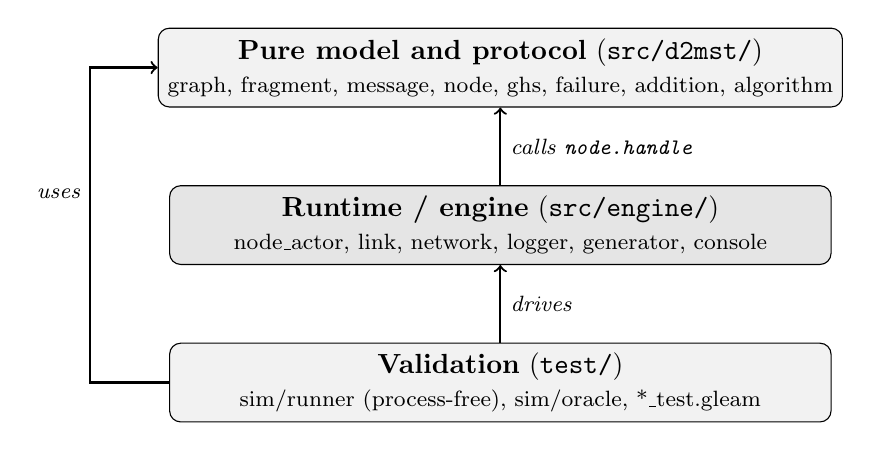
\begin{tikzpicture}[
    box/.style={draw, rounded corners, minimum width=8.4cm, minimum height=1cm, align=center},
    lbl/.style={font=\footnotesize\itshape}
]
\node[box, fill=black!5] (protocol) at (0,4) {\textbf{Pure model and protocol} (\texttt{src/d2mst/})\\
\footnotesize graph, fragment, message, node, ghs, failure, addition, algorithm};
\node[box, fill=black!10] (engine) at (0,2) {\textbf{Runtime / engine} (\texttt{src/engine/})\\
\footnotesize node\_actor, link, network, logger, generator, console};
\node[box, fill=black!5] (test) at (0,0) {\textbf{Validation} (\texttt{test/})\\
\footnotesize sim/runner (process-free), sim/oracle, *\_test.gleam};

\draw[->, thick] (test) -- node[right, lbl] {drives} (engine);
\draw[->, thick] (test.west) -- ++(-1,0) |- node[pos=0.3, left, lbl, align=right] {uses} (protocol.west);
\draw[->, thick] (engine) -- node[right, lbl] {calls \texttt{node.handle}} (protocol);
\end{tikzpicture}
\caption{The three-layer split. Protocol code has no notion of processes; the engine is
the only layer that touches them; validation exercises both, either directly or through
the process-free simulator.}
\label{fig:layers}
\end{figure}

The codebase follows the three-layer split of Figure~\ref{fig:layers}. This separation is
chosen so that the protocol, the part of the system whose correctness matters most, can be
understood, tested, and reasoned about independently of processes, scheduling, or message
loss.

\subsection{Pure model and protocol (\texttt{src/d2mst/})}

Every module in this layer is a pure function of its inputs; none of them import
\texttt{gleam/erlang/process} or \texttt{gleam/otp/actor}.

\begin{itemize}
  \item \texttt{graph.gleam}: the \texttt{Graph}, \texttt{Edge}, and symmetric
  \texttt{EdgeId(low, high)} types, together with \texttt{compare\_edge}, the
  lexicographic order on $(w(e), \mathrm{id}(e))$ that makes the MST unique regardless of
  weight collisions. This order is what allows \texttt{kruskal}, a plain union-find MST
  also defined here, to serve as an exact oracle for the distributed result.
  \item \texttt{fragment.gleam}: the \texttt{FragmentId} type (Section~\ref{sec:fragment-id}).
  \item \texttt{message.gleam}: every wire message, split into \texttt{GHSMsg} (Tier 1),
  \texttt{D2MMsg} (failure response), and \texttt{AddMsg} (addition response), together
  with the two predicates that decide which messages must carry a matching fragment
  identity to be accepted (Section~\ref{sec:intra-fragment}).
  \item \texttt{node.gleam}: the \texttt{State} record, the \texttt{Event} type
  (\texttt{Wakeup}, \texttt{Receive}, \texttt{LinkUp}, \texttt{LinkDown}), the
  \texttt{Effect} type (\texttt{Send}), and small pure helpers shared by every protocol
  module, such as looking up an edge, selecting the minimum edge satisfying a predicate,
  or deferring a message. It contains no protocol logic of its own.
  \item \texttt{ghs.gleam}, \texttt{failure.gleam}, and \texttt{addition.gleam}: the three
  protocol tiers, one module each, all operating on the same \texttt{node.State}. This
  split keeps Tier 1, 2, and 3 almost separated while letting them share state and the
  fragment-identity invariant that makes their concurrent execution safe.
  \item \texttt{algorithm.gleam}: the single exposed entry point,
  \texttt{handle(state, event) -> \#(state, effects)}. It dispatches an event to the
  appropriate tier according to the message type, and then drains the pending queue: a
  message a handler could not yet process (Section~\ref{sec:defer}) is retried after every
  subsequent event, repeatedly, until a pass makes no further progress.
\end{itemize}

\subsection{Runtime / engine (\texttt{src/engine/})} \label{sec:link-actor}

This is the only layer that touches BEAM processes, and the only place where protocol code
is driven by something other than a direct function call.

\begin{itemize}
  \item \texttt{node\_actor.gleam}: a thin actor shell, one BEAM process per graph node.
  It turns every incoming event, whether a wakeup, a received message, or a link
  appearing or disappearing, into a call to \texttt{algorithm.handle}, performs the
  returned \texttt{Send} effects by forwarding them to link actors, and reports every send
  and every resulting state to the logger. It contains no protocol logic of its own.
  \item \texttt{link.gleam}: one actor per edge, so that the process itself represents the
  edge. The system therefore has no separate representation of a failed link: deleting an
  edge means terminating this process directly, and both endpoint nodes, which monitor it,
  observe the termination as an ordinary \texttt{LinkDown} event. A link additionally
  monitors both of its endpoint nodes and stops itself as soon as either one dies, since a
  channel with only one live endpoint no longer serves any purpose. This single rule is
  what reduces a node crash to plain link failures at every neighbor, without any protocol
  code having to distinguish a peer node dying from the edge itself failing.
  \item \texttt{network.gleam}: builds a running network of node and link actors from a
  \texttt{Graph} and exposes the topology-event API used by the tests and the demo:
  \texttt{wake\_all}, \texttt{fail\_link}, \texttt{add\_link}, \texttt{crash\_node}, and
  \texttt{add\_node}. Each of these mutates the live actors and returns an updated
  \texttt{Network} whose \texttt{.graph} field reflects the new topology, so that
  assertions in the tests always compare against the graph that is actually running.
  \item \texttt{logger.gleam}: a central observer process that nodes report to on every
  state change. The protocol never depends on
  it, since it holds no protocol state of its own, only an ordered history that nodes push
  into, and its process is unlinked from the rest of the system, so that killing it does not take the network down with it.
  \item \texttt{generator.gleam}: a seeded generator and a
  connected-graph builder. It is used instead of Erlang's \texttt{:rand} specifically so
  that a failing random test, or a bad round of the interactive demo, is reproducible from
  its integer seed alone. It is also what \texttt{d2mst.gleam} uses to build graphs and to
  schedule random topology events from user-supplied counts.
  \item \texttt{console.gleam}: A thin standard-input and clock wrapper from Erlang code.
\end{itemize}

\subsection{Validation (\texttt{test/})}

\begin{itemize}
  \item \texttt{test/sim/runner.gleam}: a second, process-free runtime. A single FIFO
  queue of \texttt{\#(NodeId, Event)} drives \texttt{algorithm.handle} for every node
  until the system quiesces, all within one BEAM process. It runs the exact same protocol
  modules as the production code, only the driving loop differs, but it is deterministic
  and can be stepped one event at a time, which makes it the preferred tool for chasing a
  logic bug: a failure found here reproduces every time, with no scheduling
  nondeterminism to contend with.
  \item \texttt{test/sim/oracle.gleam}: checks a converged run against
  \texttt{graph.kruskal}. The union of reported tree edges must equal the unique MST,
  there must be exactly one root per connected component, and every parent pointer must be
  a tree edge.
  \item \texttt{test/*\_test.gleam}: Specific unit tests for the modules, and fuzz tests that drive the process-free simulator with random topology events and check the result against the oracle.
\end{itemize}

\section{Decisions made to implement the protocol}

\paragraph{Incremental construction on top of GHS.}
The implementation was built in two stages: GHS (Tier 1) first, then the dynamic
repair protocol on top of it. The dynamic protocol
needs an already-converged spanning tree to operate on, so GHS is kept in the final
system as the mechanism that constructs that initial tree, rather than being replaced
once Tier 2/3 were implemented. One consequence of this ordering is that failure and
addition events are only ever injected once GHS has converged and the tree is stable;
the two protocols were not tested interacting \emph{while} the initial tree is still
being constructed.

\paragraph{Process per edge.}
The design already calls for one logical process per network node. The implementation
takes the same idea further and gives every edge its own process as well
(Section~\ref{sec:link-actor}), rather than having node processes exchange messages
directly. As a consequence, a link failure and a node crash reduce to the same primitive
event, namely a monitored process terminating, observed from different places. The
protocol therefore only ever has to handle one case, \texttt{LinkDown}, and the
failure-transparency requirement of Chapter~\ref{ch:analysis} follows from the runtime
topology rather than requiring dedicated detection code.

\paragraph{Pure state machine.}
Every protocol handler has the shape \texttt{State -> Event -> \#(State, List(Effect))},
with \texttt{Effect} restricted to \texttt{Send(on, msg)}: no module in
\texttt{src/d2mst/} performs I/O, spawns a process, or blocks. \texttt{node\_actor.gleam}
is the only place where an \texttt{Effect} is turned into an actual message send. This
separation is what makes the process-free simulator possible: it links against the same
protocol modules and simply interprets the returned effects into its own event queue
instead of onto real links, so that a bug reproduced in the simulator is necessarily a bug
in the deployed protocol.

\paragraph{MOE search strategy selection.}
Chapter~\ref{ch:project} describes two independent Phase 3 procedures. In the
implementation they are a single type, \texttt{MoeStrategy} (\texttt{Naive} or
\texttt{BinarySearch(sample\_k)}), fixed once per node at \texttt{init} and threaded
through \texttt{failure.gleam}'s \texttt{start\_repair\_search}. Fixing the strategy at
construction time, rather than negotiating it at every repair, reflects the fact that the
choice is a deployment parameter of the whole network, not a per-event decision. It also
allows both strategies to be run against the same test and benchmark infrastructure, so
that their message counts can be compared directly.

\paragraph{Hash function.}
Chapter~\ref{ch:project}'s \textsc{TestOut} and priority-sampling steps are parameterized
by an abstract random oracle $H$. The implementation instantiates it with SHA-256
(\texttt{gleam\_crypto}), truncated to its low 64 bits and applied to the edge id
$(\min(u,v), \max(u,v))$. This is large enough that the $2^{-64}$ false-negative
probability derived in Chapter~\ref{ch:project} is negligible for any fragment size the
tests exercise, and it reuses a standard, already checked primitive rather than a custom
pseudo-random function. Each node also caches its sorted, hashed incident-edge list
(\texttt{bs\_candidates}) for the duration of one search, rebuilding it only when the
search restarts or the incident edge set changes, so that a \textsc{TestOut} round does
not re-sort and re-hash the same edges from scratch every time.


\paragraph{Interactive demo.}\label{sec:interactive-main}

\texttt{d2mst.gleam} builds a random connected graph, brings it to a converged MST, and
then repeatedly asks for a round of node and edge failures and additions, applies all of
them as one overlapping burst with nothing allowed to settle in between, waits for
convergence, and checks the result against \texttt{graph.kruskal} while reporting the
message count and wall-clock time for the round. Applying a whole batch of topology
changes at once, rather than one at a time, is deliberate: it directly validates the
protocol's ability to safely resolve the concurrent, overlapping network events detailed
in Chapter~\ref{ch:project}.

\section{Failure protocol: implementation details}

This section completes the description of the failure response protocol
given in Chapter~\ref{ch:project}. It covers implementation-level choices that were not
settled at the design stage.

\subsection{Messages by phase}\label{sec:failure-messages}

Chapter~\ref{ch:project} describes each phase of the failure response protocol without
naming the concrete messages that carry it out. The messages below, all constructors of
\texttt{D2MMsg}, are what the implementation actually sends.

\begin{itemize}
  \item \textbf{Phase 1, detection and split.} \msg{ReportFailure} carries the freshly
  generated identity from the failed edge's parent-side endpoint up toward the fragment
  root, one hop at a time.
  \item \textbf{Phase 2, re-identification.} \msg{ReIden} broadcasts the new identity down
  the tree; \msg{ReIdenAck} convergecasts the acknowledgement back up, with an internal
  node waiting for one from every child before sending its own.
  \item \textbf{Phase 3, naive search.} \msg{ProbeMoe} broadcasts down the tree to start
  every node's local search. \msg{ProbeEdge} is sent to a non-tree neighbor to ask whether
  the link between them crosses the fragment boundary, and \msg{ProbeReply} carries the
  answer back. \msg{ReportMoe} convergecasts each subtree's best candidate edge up to the
  parent.
  \item \textbf{Phase 3, binary search.} \msg{BsRound} broadcasts the start of the
  search's first, unfiltered scan of the whole fragment, and \msg{BsRoundReport}
  convergecasts each node's contribution (its XOR, edge bounds, and priority sample). Once
  an interval is known, \msg{BsSplit} broadcasts it split at the sampled median, and
  \msg{BsSplitReport} convergecasts both halves' contributions. When the interval
  collapses to a single edge, \msg{BsMoeFound} broadcasts its id so that the owning
  endpoint can claim it.
  \item \textbf{Phase 4, merge.} In the naive strategy, \msg{SignalConnect} routes the
  merge request down the tree branch that holds the MOE; the binary search strategy uses
  \msg{BsMoeFound} for the same purpose instead. \msg{Connect} is then sent by the node
  holding the MOE to its counterpart across the boundary once it marks the edge
  \texttt{Selected}. If a fragment finds no outgoing edge at all, \msg{GoSleep}
  broadcasts from the root instead, putting every node into the terminal
  \texttt{Sleeping} state.
\end{itemize}

\subsection{Fragment identity representation}\label{sec:fragment-id}

\texttt{FragmentId} has three constructors, not two:

\begin{itemize}
  \item \texttt{Singleton(node)}: a fresh, not yet merged node, at level 0, before Tier 1
  has run.
  \item \texttt{GHSCore(edge)}: a fragment created by a Tier 1 merge, identified by its
  core edge, exactly as in the original GHS paper.
  \item \texttt{D2MCore(edge, node: Option(NodeId), failures\_counter)}: a fragment
  created by the dynamic repair protocol.
\end{itemize}

The \texttt{node} field corresponds to the $u$ or $v$ that Chapter~\ref{ch:project} uses
to break the symmetry between the two identities generated when a tree edge fails: it is
set to \texttt{Some(endpoint)} exactly when the identity is produced by a split
(\texttt{remove\_edge}, Phase 1), where it distinguishes the two new fragments that share
the failed edge. A Phase 4 merge (Section~\ref{sec:phase4-impl}), by contrast, produces
exactly one new identity for the combined fragment, so there is nothing to disambiguate
and \texttt{node} is set to \texttt{None} in that case. \texttt{failures\_counter} is
$k(e)$: it is incremented every time the corresponding edge fails, so that the same edge
failing twice does not produce two identical identities.

\subsection{Fragment-identity checks on messages}\label{sec:intra-fragment}

Chapter~\ref{ch:project} states the discard rule at the level of intra-fragment messages
carrying the sender's identity, with a mismatch resulting in silent discard. In the
implementation this is not a blanket rule applied to every \texttt{D2MMsg} or
\texttt{AddMsg}: each message type is classified once, by a predicate
(\texttt{fail\_is\_intra\_fragment} for \texttt{D2MMsg}, \texttt{add\_is\_intra\_fragment}
for \texttt{AddMsg}), and only messages that are meant to stay inside one stable fragment
are checked. A few messages are exempt by design, since requiring a match would prevent
them from ever being processed:

\begin{itemize}
  \item \msg{ReportFailure} (Phase 1) must reach the root regardless of how many times the
  identity above it has already changed while it is in flight, since it is not itself a
  protocol round, only a topology notification climbing the tree.
  \item \msg{ReIden} is exempt because it is the message carrying the new identity: it
  cannot be validated against the receiver's old one.
  \item \msg{ProbeEdge}, \msg{ProbeReply}, and \msg{Connect} (Phase 3 and 4) cross the
  fragment boundary by design, since testing whether an edge is outgoing requires it: the
  sender's identity is expected to differ from the receiver's.
\end{itemize}

\subsection{Phase 3: search-state bookkeeping}\label{sec:phase3-impl}

Every repair round begins by resetting the edge bookkeeping left over from a previous
round or from the initial construction: every edge marked \texttt{Rejected} is reset to
\texttt{Undecided}, while \texttt{Selected} edges, which form the current tree, are left
untouched. This way, the search reconsiders every non-tree edge rather than trusting a
verdict reached under a different fragment shape.

The naive procedure's liveness depends on one further detail not implied by
Chapter~\ref{ch:project}: if the edge a node is currently probing
(\texttt{state.test\_edge}) is the one that just failed, the expected \msg{ProbeReply}
will never arrive. \texttt{remove\_edge} checks for this case and, when it applies,
immediately moves on to the next undecided edge instead of leaving the search stalled
waiting for a reply from a process that no longer exists.

\subsection{Phase 4: merge}\label{sec:phase4-impl}

The two fragments involved arrive independently at the same MOE, and each marks that edge
\texttt{Selected} on its own side before sending \msg{Connect}, with nothing forcing the
two sends to happen at the same time. Whichever \msg{Connect} arrives first therefore
lands on a receiver that has not yet made the same choice; that branch of
\texttt{on\_connect} simply defers the message (Section~\ref{sec:defer}) rather than
treating it as an error, and it is retried automatically once this side's own search
reaches the same edge. Only once both sides have sent and received a \msg{Connect} for the
edge does the merge proceed. Node identifiers break the symmetry exactly as in Tier 1's
core-edge merge: the smaller identifier becomes the new root and issues the next Phase 1/2
wave, while the larger identifier records the edge as its parent and clears the addition
bookkeeping in the same step (Section~\ref{sec:failure-addition}), since its own
\texttt{state.fragment} field changes at this point, before the ReIden broadcast described
in Chapter~\ref{ch:project} reaches it.


\section{Addition protocol: implementation details}

This section completes the description of the addition protocol given in Chapter~\ref{ch:project}. It covers implementation-level choices that were not
settled at the design stage.

\subsection{Interaction with the addition protocol}\label{sec:failure-addition}

Chapter~\ref{ch:project} leaves open what happens when a tree edge inside an in-progress
addition's cycle fails while the addition is still running. No dedicated coordination code
is needed for correctness: because both protocols are gated by the same fragment-identity
check (Section~\ref{sec:intra-fragment}), a failure that reassigns a fragment's identity
in the middle of an addition causes every \msg{Addition}, \msg{AddRequestTurn},
\msg{Privilege}, \msg{Replace}, and \msg{AddDone} message still travelling under the old
identity to be silently discarded as soon as it reaches a node that has already
re-identified, through the same mechanism that already protects two overlapping repairs
from each other.

What does require explicit handling is the bookkeeping that an abandoned addition round
leaves behind, since nothing else revisits it once its messages stop being delivered:

\begin{itemize}
  \item \textbf{Clearing stale state:} Whenever a node adopts a new fragment identity—such as during \texttt{start\_reiden\_phase} or the mutual merge branch of \texttt{on\_connect}, it executes \texttt{clear\_addition\_state}. This function wipes all addition-related local storage tied to the old identity, including \texttt{pending\_additions}, \texttt{turn\_routing}, and \texttt{addition\_queue}. Clearing this state prevents stale routing entries from persisting in future protocol events.
  
  \item \textbf{Tracking addition edges:} The dropped addition itself must not be permanently forgotten. When a newly established link is first registered by a node, its local \texttt{EdgeInfo} struct is flagged with \texttt{via\_addition: True}.
  
  \item \textbf{The retry:} Once the concurrent failure is fully resolved and the fragment returns to quiescence (when the root broadcasts \msg{GoSleep} via \texttt{enter\_sleep} or \texttt{on\_go\_sleep}), every node invokes \texttt{retry\_abandoned\_additions}. This routine scans the node's local edges and sends a fresh \msg{AddTest} for any edge marked \texttt{via\_addition} whose status is not \texttt{Selected}.
\end{itemize}
\chapter{Validation}\label{ch:validation}

This chapter checks the implementation against the requirements of
Chapter~\ref{ch:analysis} and the protocol described in Chapter~\ref{ch:project}. Because
the protocol's own correctness criterion is exact, a run either converges to \emph{the}
unique minimum spanning tree of the current graph or it does not, validation is built
around a single reference check applied uniformly to every scenario, rather than a
collection of hand-picked expected outputs. What differs from test to test is only how
that scenario is produced: which topology, which sequence of events, and which of the two
runtimes executes it.

\section{The correctness oracle}\label{sec:oracle}

Every test in the suite ultimately delegates its verification to a single call:
\texttt{sim/oracle.check(graph, summaries)}. This function validates a converged execution
against \texttt{graph.kruskal} and accepts the run if and only if all four of the
following hold:

\begin{itemize}
  \item \textbf{Quiescence:} Every node reports \texttt{halted: True}, guaranteeing that
  the protocol reached stability;
  \item \textbf{Edge Set:} The union of all locally reported tree edges is identical to
  the exact edge set produced by \texttt{kruskal};
  \item \textbf{Root Count:} The number of nodes reporting \texttt{parent: None} equals
  the exact number of connected components in the current graph, ensuring precisely one
  root per fragment;
  \item \textbf{Structural Integrity:} Every non-root node's parent pointer connects to an
  active tree edge, confirming that directed parent references form a valid rooted forest.
\end{itemize}

Because the total edge ordering resolves all weight ties, the reference MST is strictly
unique: there is exactly one valid topology and edge set that the oracle will accept.

\section{Two execution paths, one protocol}

Every test drives one of two runtimes: the real OTP
actor system, or \texttt{test/sim/runner.gleam}'s process-free simulator. Both call exactly
the same \texttt{d2mst/algorithm.handle} on exactly the same protocol modules; the only
difference is what delivers events to it. The simulator interprets a node's \texttt{Send}
effects directly into its own FIFO queue instead of onto a real link process, and lets a
scenario be driven completely deterministically: the same sequence of \texttt{wake},
\texttt{fail\_link}, \texttt{add\_link}, and \texttt{crash\_node} calls produces the exact
same interleaving of events every time, and can be stepped one message at a time with
\texttt{step\_one}.

The actor runtime is not redundant with this. It is the only place where a
\texttt{LinkDown} is an actual monitored BEAM process dying, rather than an event handed
directly to the queue, and the only place where two nodes' handlers genuinely run
concurrently instead of being serialized by a single driving loop. Section~\ref{sec:actor}
describes what it is used to check that the simulator structurally cannot.

\section{Randomized and regression testing}\label{sec:fuzz}

Fixed graphs catch bugs that are wrong for every input; they are not good for bugs that
depend on a particular tree shape or a particular pair of overlapping events. To avoid this 
\texttt{engine/generator.gleam} implements a seeded connected-graph builder: the same seed 
always produces the same graph, so a fuzz failure is reproducible from its integer seed with 
no additional state to capture. Most fuzz tests follow the same shape: converge on a batch 
of seeded topologies, apply a scenario, and check the oracle after every one.

A second group of tests fires several topology events \emph{without settling in between},
so that their protocol rounds are genuinely concurrent and not just sequential with no gap.

The most targeted tests are fixed, hand-built
graphs written to reconstruct a specific race the general-purpose fuzzing above did not
happen to find, and are kept as permanent regression tests once the underlying bug is
fixed. For example \texttt{overlapping\_cycles\_test} builds two link additions whose cycles genuinely
share tree edges, exactly the race Chapter~\ref{ch:project}'s "overlapping cycles
serialization" paragraph describes.

\section{Long-running randomized simulation}\label{sec:long-running}

Chapter~\ref{ch:intro}'s system overview commits the evaluation to, among other scenarios,
"concurrent random additions and deletions" and "long-running simulations with node and
edge events occurring at different rates". \texttt{long\_running\_random\_topology\_test}
is built directly for this: starting from a five-hundred-node random graph, it fires sixty
topology events, drawn uniformly across failing a random edge, crashing a random node,
adding a random edge, and joining a new isolated node, biased against crashing below five
surviving nodes so the run always has something left to mutate, in bursts of five with
\emph{nothing allowed to settle in between}. The oracle of Section~\ref{sec:oracle} is
checked after every burst, so a burst of five overlapping events
must both leave the system in a checkable state and eventually converge correctly, not just
the final one. \texttt{fuzz\_long\_running\_random\_topology\_test} repeats the same
procedure from five different starting topologies. 

\section{Interactive demonstration}

\texttt{gleam run} (Appendix~\ref{app:devenv}) is not part of the automated suite, but
complements it: it builds a random connected graph, brings it to a converged MST, and then
repeatedly applies
a whole batch of node and edge failures and additions as one overlapping burst, waits for
convergence, checks the result against \texttt{graph.kruskal}, and reports the message
count and wall-clock time for the round.

\section{Message-complexity benchmark}\label{sec:bench}

Chapter~\ref{ch:project} derives $O(|E|)$ message complexity for the naive Phase 3 search
and $O(N \log N)$ for the binary-search alternative. \texttt{test/bench\_report.gleam} is
not a \texttt{gleeunit} test, it can be run with:

{\footnotesize
\begin{verbatim}
gleam build --target erlang
erl -pa build/dev/erlang/*/ebin -noshell \
  -eval "bench_report:run(), halt()."
\end{verbatim}
}

For each graph size $N \in \{10, 20, 40, 80, 160, 320\}$ and each burst size $k \in \{1, 2,
4, 8, 16\}$ (how many tree edges, or non-adjacent pairs, are perturbed at once before the
network is allowed to settle), the benchmark builds \texttt{seed\_count} $= 15$ random
graphs, runs the scenario, measures the messages sent between before and after the burst,
and reports the mean alongside its ratio to the complexity claim's asymptotic term: mean
$|E|$ for the naive search, $N \log_2 N$ for the binary search, and $N$ for the addition
protocol. Failure scenarios are measured at two densities, a sparse graph
($\mathrm{edge\_pct} = 15$) and a dense one ($\mathrm{edge\_pct} = 85$), since the naive
bound is stated in terms of $|E|$ and the two densities are where that quantity differs
most from $N$.
The full sweep, one table per scenario:

{\footnotesize
\begin{verbatim}
Failure - naive Phase 3, sparse (edge_pct=15)
N              k=1           k=2            k=4            k=8            k=16
--------------------------------------------------------------------------------
N=10     111.0 (7.9x)  132.8 (9.5x)  150.7 (10.8x)  106.4 (7.6x)              n/a
N=20     334.7 (7.3x) 477.1 (10.5x)  683.8 (15.0x)  863.0 (18.9x)  899.4 (19.7x)
N=40    1105.0 (7.4x) 1549.5 (10.3x) 2436.1 (16.3x) 3471.3 (23.2x) 4795.3 (32.0x)
N=80    3941.5 (7.3x) 5580.8 (10.3x) 8483.7 (15.7x) 12171.3 (22.5x) 17930.3 (33.1x)
N=160  13979.1 (6.8x) 20334.7 (9.9x) 29249.5 (14.3x) 46246.5 (22.6x) 68519.5 (33.4x)
N=320  53579.5 (6.7x) 75717.4 (9.5x) 112743.7 (14.1x) 172983.5 (21.7x) 258182.9 (32.4x)

Failure - naive Phase 3, dense (edge_pct=85)
N              k=1           k=2            k=4            k=8            k=16
--------------------------------------------------------------------------------
N=10     265.6 (6.7x)  333.8 (8.4x)  399.3 (10.0x)  427.1 (10.8x)             n/a
N=20    1011.6 (6.2x) 1229.9 (7.5x)  1565.5 (9.6x) 1926.9 (11.8x) 2140.8 (13.1x)
N=40    3980.8 (6.0x) 4922.5 (7.4x)  6325.5 (9.5x) 8036.7 (12.1x) 9816.5 (14.7x)
N=80   14937.9 (5.5x) 18422.4 (6.8x) 22465.1 (8.3x) 28189.5 (10.4x) 36704.1 (13.6x)
N=160  64180.2 (5.9x) 73621.7 (6.8x) 93659.2 (8.6x) 110659.1 (10.2x) 143435.5 (13.2x)
N=320 241979.6 (5.6x) 311050.5 (7.2x) 368015.0 (8.5x) 456982.8 (10.5x) 577752.4 (13.3x)

Failure - binary search Phase 3, sparse (edge_pct=15)
N              k=1           k=2            k=4            k=8            k=16
--------------------------------------------------------------------------------
N=10     119.6 (3.6x)  151.5 (4.6x)  173.3 (5.2x)  117.6 (3.5x)              n/a
N=20     345.9 (4.0x)  571.8 (6.6x)  979.9 (11.3x) 1428.3 (16.5x) 1635.6 (18.9x)
N=40    1044.3 (4.9x) 1793.1 (8.4x) 3258.5 (15.3x) 5372.4 (25.2x) 8383.4 (39.4x)
N=80    2587.9 (5.1x) 4742.0 (9.4x) 8891.1 (17.6x) 15617.3 (30.9x) 26616.7 (52.6x)
N=160   5699.9 (4.9x) 10948.5 (9.3x) 21327.9 (18.2x) 40897.2 (34.9x) 73864.5 (63.1x)
N=320  13499.3 (5.1x) 26275.0 (9.9x) 50914.7 (19.1x) 97952.9 (36.8x) 186660.3 (70.1x)

Failure - binary search Phase 3, dense (edge_pct=85)
N              k=1           k=2            k=4            k=8            k=16
--------------------------------------------------------------------------------
N=10     187.8 (5.7x)  297.0 (8.9x)  424.6 (12.8x)  479.5 (14.4x)             n/a
N=20     518.7 (6.0x) 881.5 (10.2x) 1545.9 (17.9x) 2232.6 (25.8x) 2806.1 (32.5x)
N=40    1326.1 (6.2x) 2412.9 (11.3x) 4407.7 (20.7x) 7547.1 (35.5x) 11555.8 (54.3x)
N=80    3178.1 (6.3x) 5700.4 (11.3x) 10558.1 (20.9x) 18427.5 (36.4x) 31333.2 (62.0x)
N=160   6882.9 (5.9x) 13367.6 (11.4x) 26449.0 (22.6x) 49068.5 (41.9x) 89685.5 (76.6x)
N=320  15734.3 (5.9x) 30885.2 (11.6x) 59553.6 (22.4x) 114585.3 (43.0x) 220605.3 (82.8x)

Addition, edge_pct=40
N              k=1           k=2            k=4            k=8            k=16
--------------------------------------------------------------------------------
N=10      26.7 (2.7x)  55.2 (5.5x)  111.1 (11.1x)  217.7 (21.8x)   438.0 (43.8x)
N=20      40.6 (2.0x)  84.4 (4.2x)   165.1 (8.3x)  333.6 (16.7x)   678.1 (33.9x)
N=40      76.8 (1.9x) 147.5 (3.7x)   297.5 (7.4x)  595.9 (14.9x)  1194.7 (29.9x)
N=80     129.3 (1.6x) 251.7 (3.1x)   500.5 (6.3x)  994.1 (12.4x)  2041.7 (25.5x)
N=160    227.7 (1.4x) 454.0 (2.8x)   894.3 (5.6x) 1774.6 (11.1x)  3534.5 (22.1x)
N=320    410.1 (1.3x) 812.1 (2.5x)  1613.9 (5.0x) 3254.2 (10.2x)  6452.5 (20.2x)
\end{verbatim}
}

At the lowest concurrency, $k=1$, a single isolated event, which is what
Chapter~\ref{ch:project}'s complexity derivations actually analyze, both failure tables'
ratio columns stay close to a constant as $N$ grows by a factor of thirty-two, from $N=10$
to $N=320$ (naive: roughly $5.5$-$8\times$ in both densities; binary search: roughly
$4$–$6.3\times$, excluding the $N=10$ sparse outlier discussed below), which is exactly what
an $O(|E|)$ and an $O(N \log N)$ bound respectively predict. The naive/binary-search
comparison also confirms the motivation Chapter~\ref{ch:project} gives for the binary-search
procedure in the first place: at $N=160$, binary search sends $5700$ messages against the
naive search's $13979$ in the sparse graph ($2.5\times$ fewer), and $6883$ against
$64180$ in the dense one ($9.3\times$ fewer). The gap widens
with $N$ too: at $N=320$ binary search is $4.0\times$ fewer messages in the sparse graph and
$15.4\times$ fewer in the dense one, both wider than at $N=160$. At the
smallest size, $N=10$, the two are close and binary search is even marginally more expensive
in the sparse case ($119.6$ against $111.0$): the extra broadcast/convergecast rounds that
selecting a median a few times costs are not yet paid back by a saving on $|E|$ that is
still tiny at that size, so the asymptotically better procedure only earns its keep once the
graph is large enough.

The ratio columns tell us something different. For naive, the $k=8$ ratio climbs with $N$ only up to a point and then flattens:
$7.6\times$, $18.9\times$, $23.2\times$, $22.5\times$, $22.6\times$, $21.7\times$ across
$N=10,\dots,320$ in the sparse graph, and just $10.8\times$-$13.6\times$ across the same
range in the dense one; the $k=16$ column repeats the same shape one notch higher, settling
around $32$-$33\times$ sparse and $13$-$15\times$ dense from $N=80$ onward. Binary search
never settles: its $k=8$ ratio keeps climbing across the whole range, from $3.5\times$ to
$36.8\times$ sparse and $14.4\times$ to $43.0\times$ dense, and $k=16$ climbs even more
steeply, reaching $70.1\times$ sparse and $82.8\times$ dense at $N=320$. Both bounds are derived for a single, isolated repair event, so this divergence is itself
evidence that concurrency affects the two strategies differently. Firing $k$ failures without letting
the system settle in between means a fragment identity change from one repair can hit a
Phase 3 search already in flight for another, and the implementation restarts such a search
from scratch.

Naive's Phase 3 search completes in one broadcast-down/convergecast-up pass, so it is
exposed to this risk only briefly, and a restart repeats work of the same order as the
search itself, $O(|E|)$. Binary search instead narrows its candidate interval across
several sequential broadcast/convergecast rounds, and a restart
discards that narrowed $[a,b]$ interval along with the sample built up over it, forcing the
search to begin again from an unfiltered scan. A search that stays in flight for more
rounds is exposed to invalidation for longer, and larger fragments need more such round,
which would explain why the binary-search ratio keeps growing with $N$ where naive's does
not.

The addition table shows the opposite trend under concurrency: at $k=8$ the ratio to $N$
\emph{falls} as $N$ grows, from $21.8\times$ at $N=10$ to $10.2\times$ at $N=320$, at
$k=16$ it falls from $43.8\times$ to $20.2\times$, and at $k=1$ it falls from $2.7\times$ to
$1.3\times$, comfortably inside the $O(N)$ bound at every cell. This matches the addition
protocol's different answer to concurrency: rather than letting an in-progress search be
invalidated and restarted, same-fragment additions are serialized one at a time behind the
root's \msg{Privilege} token (Chapter~\ref{ch:project}'s "overlapping cycles
serialization"), so $k$ concurrent additions cost closer to $k$ times one addition's cost
plus a fixed coordination overhead, rather than $k$ searches each separately paying a
restart penalty that grows with how large a fraction of the fragment's search state a
restart invalidates.

\section{Coverage against the requirements of Chapter~\ref{ch:analysis}}

Fault tolerance and eventual convergence are what the oracle of Section~\ref{sec:oracle}
checks directly, on every scenario in this chapter; partition tolerance is exercised by
every test in which a crash or failure actually disconnects the graph and the oracle still
requires exactly one root per surviving component. Failure transparency follows from
Section~\ref{sec:actor}'s process-death tests: a node never has to distinguish a crashed
neighbor from a plain link failure, because \texttt{link.gleam} already reduced one to the
other before the protocol saw an event. Concurrency transparency is the specific target of
Section~\ref{sec:fuzz}'s overlapping-event tests and Section~\ref{sec:long-running}.


\chapter{Conclusions}

What has been done with respect to what has been promised in Chapters~\ref{ch:intro} and \ref{ch:analysis}, and what is left out.

\appendix

\chapter{Appendix}

In the Appendix you can put code snippets, snapshots, installation instructions, etc.


\chapter*{Evaluation}
Your system will be judged mainly on how it operates as a distributed system. The primary evaluation will be according to whether your system has the following attributes:
\begin{itemize}
\item  It should be an interesting distributed system, making use of some of the algorithms we have covered in class for distributed synchronization, replication, fault tolerance and recovery, security, etc.
\item The software should be well designed and well implemented, in terms of the overall architecture and the detailed realization.
\item You should devise and apply systematic testing procedures, at both the unit and systems levels.
\item The system should operate reliably and with good performance, even in the face of failures.
\end{itemize}
Important, but secondary considerations include:
\begin{itemize}
\item Time taken to do the project (the sooner the better, but do not miss details in order to end sooner)
\item  How nice is the application's appearance: does it have a nice interface or a compelling visual display?
\end{itemize}

\nocite{*}
\bibliographystyle{plain}
\bibliography{../bibliography}

\end{document}